\documentclass[12pt]{amsart}
\usepackage[left=0.75in,top=0.6in,right=0.75in,bottom=0.6in]{geometry}
\usepackage{graphicx}

\begin{document}
\title{Homework 1}
\author{Sean Richardson, Economic Development}
\maketitle

\begin{enumerate}
    \item \begin{enumerate}
            \item Roland suggests taking the cheapest basket
                of food that provides $2000$ calories per day. Then, the
                poverty line is defined by the price of this basket of
                goods.
            \item The poverty gap sums over the distance between the
                poverty line $z$ and the income $y_i$ for the number of
                people under the poverty line $q$. The average poverty gap
                considers the same quantity but divides the total by the
                total amount of people $n$. Or,
                \begin{equation*}
                PG = \sum_{i=0}^q \left( \frac{z-y_i}{z} \right)
                \text{  and  } 
                APG = \sum_{i=0}^q \left( \frac{z-y_i}{z} \right)
                \end{equation*}
                The poverty gap allows for measure of not just how many are
                in poverty, but how much are in poverty on average.
            \item Measuring poverty allows the government to set econcrete
                goals for relieving poverty, which encourages effective
                policy. And, this allows NGOs/governments to measure what
                strategies for relieving poverty work best.
        \end{enumerate}
    \item \begin{enumerate}
        \item 
            Using midpoint method, we have $Y = \frac{Y_f + Y_i}{2} =
             1050000$, $\Delta Y = Y_f-Y_i = 
            600000$, $D = \frac{D_f + D_i}{2} = 537.5$, and $\Delta D =
            D_f-D_i = 55$. Then,
            \begin{equation*}
                Elasticity = \frac{Y}{D} \cdot \frac{\Delta D}{\Delta Y} =
                \frac{1050000}{600000}\cdot\frac{55}{537.5} = 0.179
            \end{equation*}
        \item This elasticity is above $0$, so the income elasticity is
            inelastic. This means that the good is a normal good.
        \item If the local government were to subsidize grain, there would
            be an increase in demand grain (because it is a normal good)
            and a decrease in demand for other goods.
    \end{enumerate}
    \item \begin{enumerate}
        \item   Bangladesh: \\
            Life Expectancy: $H = \frac{Actual-Min}{Max-Min} =
            \frac{69-20}{83-20} = 0.777$\\
            Income: $I = \frac{\ln(Actual)-\ln(Min)}{\ln(Max)-\ln(Min)} = 
            \frac{\ln(1910)-\ln(100)}{\ln(48820)-\ln(100)} = 0.476$\\
            Average Education: $EA = \frac{Actual-Min}{Max-Min} =
            \frac{8-0}{13.2-0} = 0.606$\\
            Expected Education: $EE = \frac{Actual-Min}{Max-Min} =
            \frac{10-0}{18-0} = 0.555$\\
            Education: $E = \frac{EA+EE}{2} =
            \frac{0.606+0.555}{2}=0.580$\\
            $HDI = (HEI)^{1/3} = (0.777 \cdot 0.580 \cdot 0.476)^{1/3} =
            0.599$\\

            Niger:\\
            Life Expectancy: $H = \frac{Actual-Min}{Max-Min} =
            \frac{55-20}{83-20} = 0.555$\\
            Income: $I = \frac{\ln(Actual)-\ln(Min)}{\ln(Max)-\ln(Min)} = 
            \frac{\ln(600)-\ln(100)}{\ln(48820)-\ln(100)} = 0.289$\\
            Average Education: $EA = \frac{Actual-Min}{Max-Min} =
            \frac{5-0}{13.2-0} = 0.378$\\
            Expected Education: $EE = \frac{Actual-Min}{Max-Min} =
            \frac{7-0}{18-0} = 0.388$\\
            Education: $E = \frac{EA+EE}{2} =
            \frac{0.378+0.388}{2}=0.383$\\
            $HDI = (HEI)^{1/3} = (0.555 \cdot 0.383 \cdot 0.289)^{1/3} =
            0.397$

        \item The life expectancy, education, and per-capita income is
            better in Bangladesh than in Niger. And, the HDI is higher in
            Bangladesh than in Niger, so it seems like a good measurement.
    \end{enumerate}
    \item \begin{enumerate}
        \item I found:\\
            headcount ratio = $0.2$; poverty gap index = $0.11488$; poverty
            severity index = $0.082$.\\
            Poverty is not uncommon (being $20\%$), but there is one case
            of a household being far below the poverty line so it could be
            called severe.\\
            Note: the poverty line was given per person and the incomes
            were given per household, so I multiplied the per person
            poverty line by the average household size $4.8$ to get a
            household poverty line.
        \item After the 100 rupee transfer, I found:
            headcount ratio = $0.1$; poverty gap index = $0.0565$; poverty
            severity index = $0.0320$.\\
            The direct transfer of money decreased all three index measures
            of poverty.
        \item~\\\begin{center}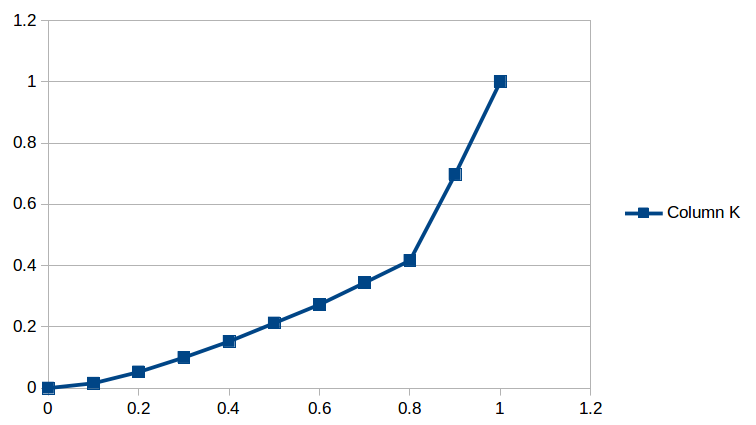
\includegraphics[width=0.7\textwidth]{lorentz_curve.png}\end{center}
        \item I calculated the Gini coefficient to be: $0.449$. This is
            high for India, for India's average Gini in 2013 is $0.34$.
            But, this is not as high as Kenya's Gini coefficient in 2013 of
            $0.48$
    \end{enumerate}
\end{enumerate}

\end{document}
